% Template file for an a0 portrait poster.
% Written by Graeme, 2001-03 based on his SOC poster.
%
% See discussion and documentation at
% <http://www.astro.gla.ac.uk/users/norman/docs/posters/> 
%
%%%%%%%%%%%%%%%%%%%%%%%%%%%%%%%%%%%%%%%%
% Modified by Jozef Dobo\v{s} (c) 2011 % 
%%%%%%%%%%%%%%%%%%%%%%%%%%%%%%%%%%%%%%%%

\documentclass[a1,portrait]{a1poster}
% You might find the 'draft' option to a0 poster useful if you have
% lots of graphics, because they can take some time to process and
% display. (\documentclass[a0,draft]{a0poster})

\pagestyle{empty}
\setcounter{secnumdepth}{0}
\usepackage[absolute]{textpos}
\usepackage{wrapfig,times}
\usepackage{graphicx}
\usepackage{forloop}
\usepackage[margin=0cm]{geometry}
%\usepackage{framed,color}
\usepackage{tikz}
\usetikzlibrary{shapes,snakes}
\usepackage{setspace}
\usepackage{bm}
\usepackage[varg]{txfonts}
\usepackage{rotating}


\usepackage{color}
\usepackage[colorlinks, pdfborder={0 0 0}]{hyperref}
\definecolor{LinkColor}{rgb}{0.75, 0, 0}
\definecolor{CiteColor}{rgb}{0, 0.5, 0.5}
\definecolor{UrlColor}{rgb}{0, 0, 0.75}
\hypersetup{linkcolor=LinkColor}
\hypersetup{citecolor=CiteColor}
\hypersetup{urlcolor=UrlColor}
\DeclareMathAlphabet{\mathpzc}{OT1}{pzc}{m}{it}



%%%%%%%%%%
% Colors %
%%%%%%%%%%
\usepackage{color}
\definecolor{TitleColor}{rgb}{1,1,1} % white
\definecolor{BannerOneColor}{rgb}{0,0,0} % pitch black
\definecolor{BannerTwoColor}{rgb}{0.93,0.08,0.31} % pinky red
\definecolor{BannerThreeColor}{rgb}{0,0.27,0.48} % dark blue
\definecolor{BannerFourColor}{rgb}{0.33,0.19,0.098} % brown
\definecolor{BannerFiveColor}{rgb}{.93,0.,0.03} % some shade in red
\definecolor{BannerSixColor}{rgb}{0,0.27,0.42} % dark blue
\definecolor{BannerSevenColor}{rgb}{0.62,0.77,0.86} % sky blue
\definecolor{BannerEightColor}{rgb}{0.35,0.33,0.01} % military green
\definecolor{BannerNineColor}{rgb}{0.85,0.86,0.34} % lime green
\definecolor{BannerTenColor}{rgb}{0,0.66,0.80} % strong blue
\definecolor{BannerElevenColor}{rgb}{0.46,0,0.20} % maroon
\definecolor{BannerTwelveColor}{rgb}{0.37,0.32,0.44} % dark washed violet
\definecolor{BannerThirteenColor}{rgb}{0.79,0.84,0.65} % light washed green
\definecolor{BannerFourteenColor}{rgb}{0.57,0.64,0.27} % dark washed green
\definecolor{BannerFifteenColor}{rgb}{0.92,0.91,0.88} % unusable washed 
\definecolor{BannerSixteenColor}{rgb}{0.97,0.36,0.14} % strong orange
\definecolor{BannerSeventeenColor}{rgb}{0.97,0.61,0.19} % orange
\definecolor{BannerEighteenColor}{rgb}{0.99,0.76,0.11} % mustard yellow
\definecolor{BannerNineteenColor}{rgb}{0.79,0.76,0.73} % light gray-ish
\definecolor{BannerTwentyColor}{rgb}{0.63,0.58,0.54} % dark gray-ish

\definecolor{shadecolor}{rgb}{0.92,0.91,0.88} % unusable washed 
%%%%%%%%%%%%%%%%%%%%%%%%%%%%%%%%%%%%%%%%%%%%%%%%%%%%%%
% Only change here to affect all headings            %
\newcommand{\headingcolor}{\color{BannerElevenColor}} 
\newcommand{\FFe}{\mathrm{FF}_\mathrm{eff}}
\newcommand{\FF}{\mathrm{FF}}
\newcommand{\blambda}{\bm{\lambda}}
\newcommand{\rhosubopt}{\rho_\mathrm{subopt}}
\newcommand{\rhoopt}{\rho_\mathrm{opt}}
\renewcommand{\figurename}{Fig.}
\newcommand{\hlm}{\mathpzc{h}_{\ell m}}

\newcommand{\ajith}[1]{\textcolor{cyan}{\textit{Ajith:#1}}}

%%%%%%%%%%%%%%%%%%%%%%%%%%%%%%%%%%%%%%%%%%%%%%%%%%%%%%

% see documentation for a0poster class for the size options here
%\let\Textsize\normalsize
\let\Textsize\Large
\def\Head#1{\noindent\hbox to \hsize{\hfil{\LARGE \headingcolor #1}}\bigskip}
\def\LHead#1{\noindent{\LARGE \headingcolor #1}\smallskip}
\def\Authors#1{\noindent{\large#1}\smallskip}
\def\Subhead#1{\noindent{\large \headingcolor #1}}
\def\Title#1{\noindent{\huge #1}}

% define the color of the emphasis text here. Please use a text color 
% consistent with the color scheme of the poster 
\def\emphasis#1{{\large \color{BannerTwoColor} {#1}}}	

% Set up the grid
%
% Note that [0cm,0cm] is the margin round the edge of the page --
% it is _not_ the grid size. That is always defined as 
% PAGE_WIDTH/HGRID and PAGE_HEIGHT/VGRID. In this case we use
% 25 x 25. This gives us three wide columns for text (7 grid
% spacings) and four narrow columns (1 each) at each side of these 
% text columns
%
% Note however that texblocks can be positioned fractionally as well,
% so really any convenient grid size can be used.
%

% [margin, margin]{rows}{cols}
\TPGrid[0cm,0cm]{17}{25}  % 1 - 7 - 1 - 7 - 1 Columns


% Mess with these as you like
\parindent=0pt
%\parindent=1cm
\parskip=0.5\baselineskip
\linespread{1.1}

% abbreviations
\newcommand{\ddd}{\,\mathrm{d}}

\begin{document}

% Understanding textblocks is the key to being able to do a poster in
% LaTeX. In
%
%    \begin{textblock}{width}(x,y)
%    ...
%    \end{textblock}
%
% the first argument gives the block width in units of the grid
% cells specified above in \TPGrid; the second gives the (x,y)
% position on the grid, with the y axis pointing down.

%%%%%%%%%%%%%%
% Top Banner %
%%%%%%%%%%%%%%
% if you change this part, you can get matching color for headings
% in Colors section above


\begin{textblock}{25}(0,0)
%\includegraphics[width=\paperwidth]{banners/banner11.pdf}
\colorbox{BannerElevenColor}{\parbox[c][0.07\textwidth][c]{1.0\textwidth}{\rule{\linewidth}{0pt}}}
%\includegraphics[height=2.6in]{banners/banner11.pdf}
\end{textblock}




%%%%%%%%%%%%%%%%%%%%%%%%%%%%%%%%%%%%%%%%%%%%%%%%%%%%%%%%%%%%%%%%%%%%%%%%%
%%%%%%%%%%%%%%%%%%%%%%%%%%%%%%%%%% Title %%%%%%%%%%%%%%%%%%%%%%%%%%%%%%%%
%%%%%%%%%%%%%%%%%%%%%%%%%%%%%%%%%%%%%%%%%%%%%%%%%%%%%%%%%%%%%%%%%%%%%%%%%
\begin{textblock}{15}(0.75,0.4)	 % syntax: {colum_width} (x_coordinate, y_coordinate)
{\color{TitleColor}

\Title{Constraining properties of black hole mimickers with gravitational wave observations of binary black holes}}
\end{textblock}

\begin{textblock}{23}(0.75,2.2)
\Authors{\textbf{Aditya Vijaykumar}$^1$, ~Nathan Johnson-McDaniel$^2$, ~Rahul Kashyap$^3$, ~Arunava Mukherjee$^4$, ~Parameswaran Ajith$^{1,5}$} \\ 
\textit{$^1$ International Centre for Theoretical Sciences, Tata Institute of Fundamental Research, Bengaluru 560089, India} \\
\textit{$^{2}$ Department of Applied Mathematics and Theoretical Physics, Centre for Mathematical Sciences, University of Cambridge, Cambridge, CB3 0WA, United Kingdom} \\
\textit{$^{3}$ The Pennsylvania State University, University Park, Pennsylvania 16802, USA} \\
\textit{$^{4}$ Astroparticle Physics and Cosmology Division, Saha Institute of Nuclear Physics, 1/AF Bidhannagar, Kolkata-700064, India} \\
\textit{$^{5}$ Canadian Institute for Advanced Research, CIFAR Azrieli Global Scholar, MaRS Centre, West Tower, 661 University Ave., Suite 505, Toronto, ON M5G 1M1, Canada} \\
\end{textblock}
%%%%%%%%%%%%%%%%%%%%%%%%%%%%%%%%%%%%%%%%%%%%%%%%%%%%%%%%%%%%%%%%%%%%%%%%%


%%%%%%%%%%%%%%%%%%%%%% An example text block %%%%%%%%%%%%%%%%%%%%%%%%%%%%
%%%%%%%%%%%%%%%%%%%%%%%%%%%%%%%%%%%%%%%%%%%%%%%%%%%%%%%%%%%%%%%%%%%%%%%%%
\begin{textblock}{7}(1,4.3)  
% syntax: {colum_width} (x_coordinate, y_coordinate) in inches
% Please do not change the column_width and x_coordinate
  %\LHead{Introduction}
\begin{spacing}{3}
\emphasis{LIGO and Virgo have recently observed a number of gravitational wave (GW) signals that are fully consistent with being emitted by binary black holes described by general relativity. However, there are theoretical proposals of exotic objects that can be massive and compact enough to be easily confused with black holes. Nevertheless, these objects differ from black holes in having nonzero tidal deformabilities, which can allow one to distinguish binaries containing such objects from binary black holes using GW observations. Using full Bayesian parameter estimation, we constrain the parameter space of such “black hole mimickers” with binary black hole observations from the Gravitational Wave Transient Catalog - 1 (GWTC-1).}
\end{spacing}

\end{textblock}
%%%%%%%%%%%%%%%%%%%%%%%%%%%%%%%%%%%%%%%%%%%%%%%%%%%%%%%%%%%%%%%%%%%%%%%%%
%%%%%%%%%%%%%%%%%%%%%% An example text block %%%%%%%%%%%%%%%%%%%%%%%%%%%%
%%%%%%%%%%%%%%%%%%%%%%%%%%%%%%%%%%%%%%%%%%%%%%%%%%%%%%%%%%%%%%%%%%%%%%%%%

\begin{textblock}{7}(1,9.8)	% syntax: {colum_width} (x_coordinate, y_coordinate) in inches
\LHead{Background}

Black holes in binaries emit gravitational waves (GWs) in a characteristic \textit{chirp} signal; the frequency and amplitude of these signals increase with time until they merge. So far, the LIGO-Virgo Collaboration has detected 10 binary black hole (BBH) events spread over two observing runs. The third observing run in currently ongoing.
\begin{figure*}[t]
	\centering
	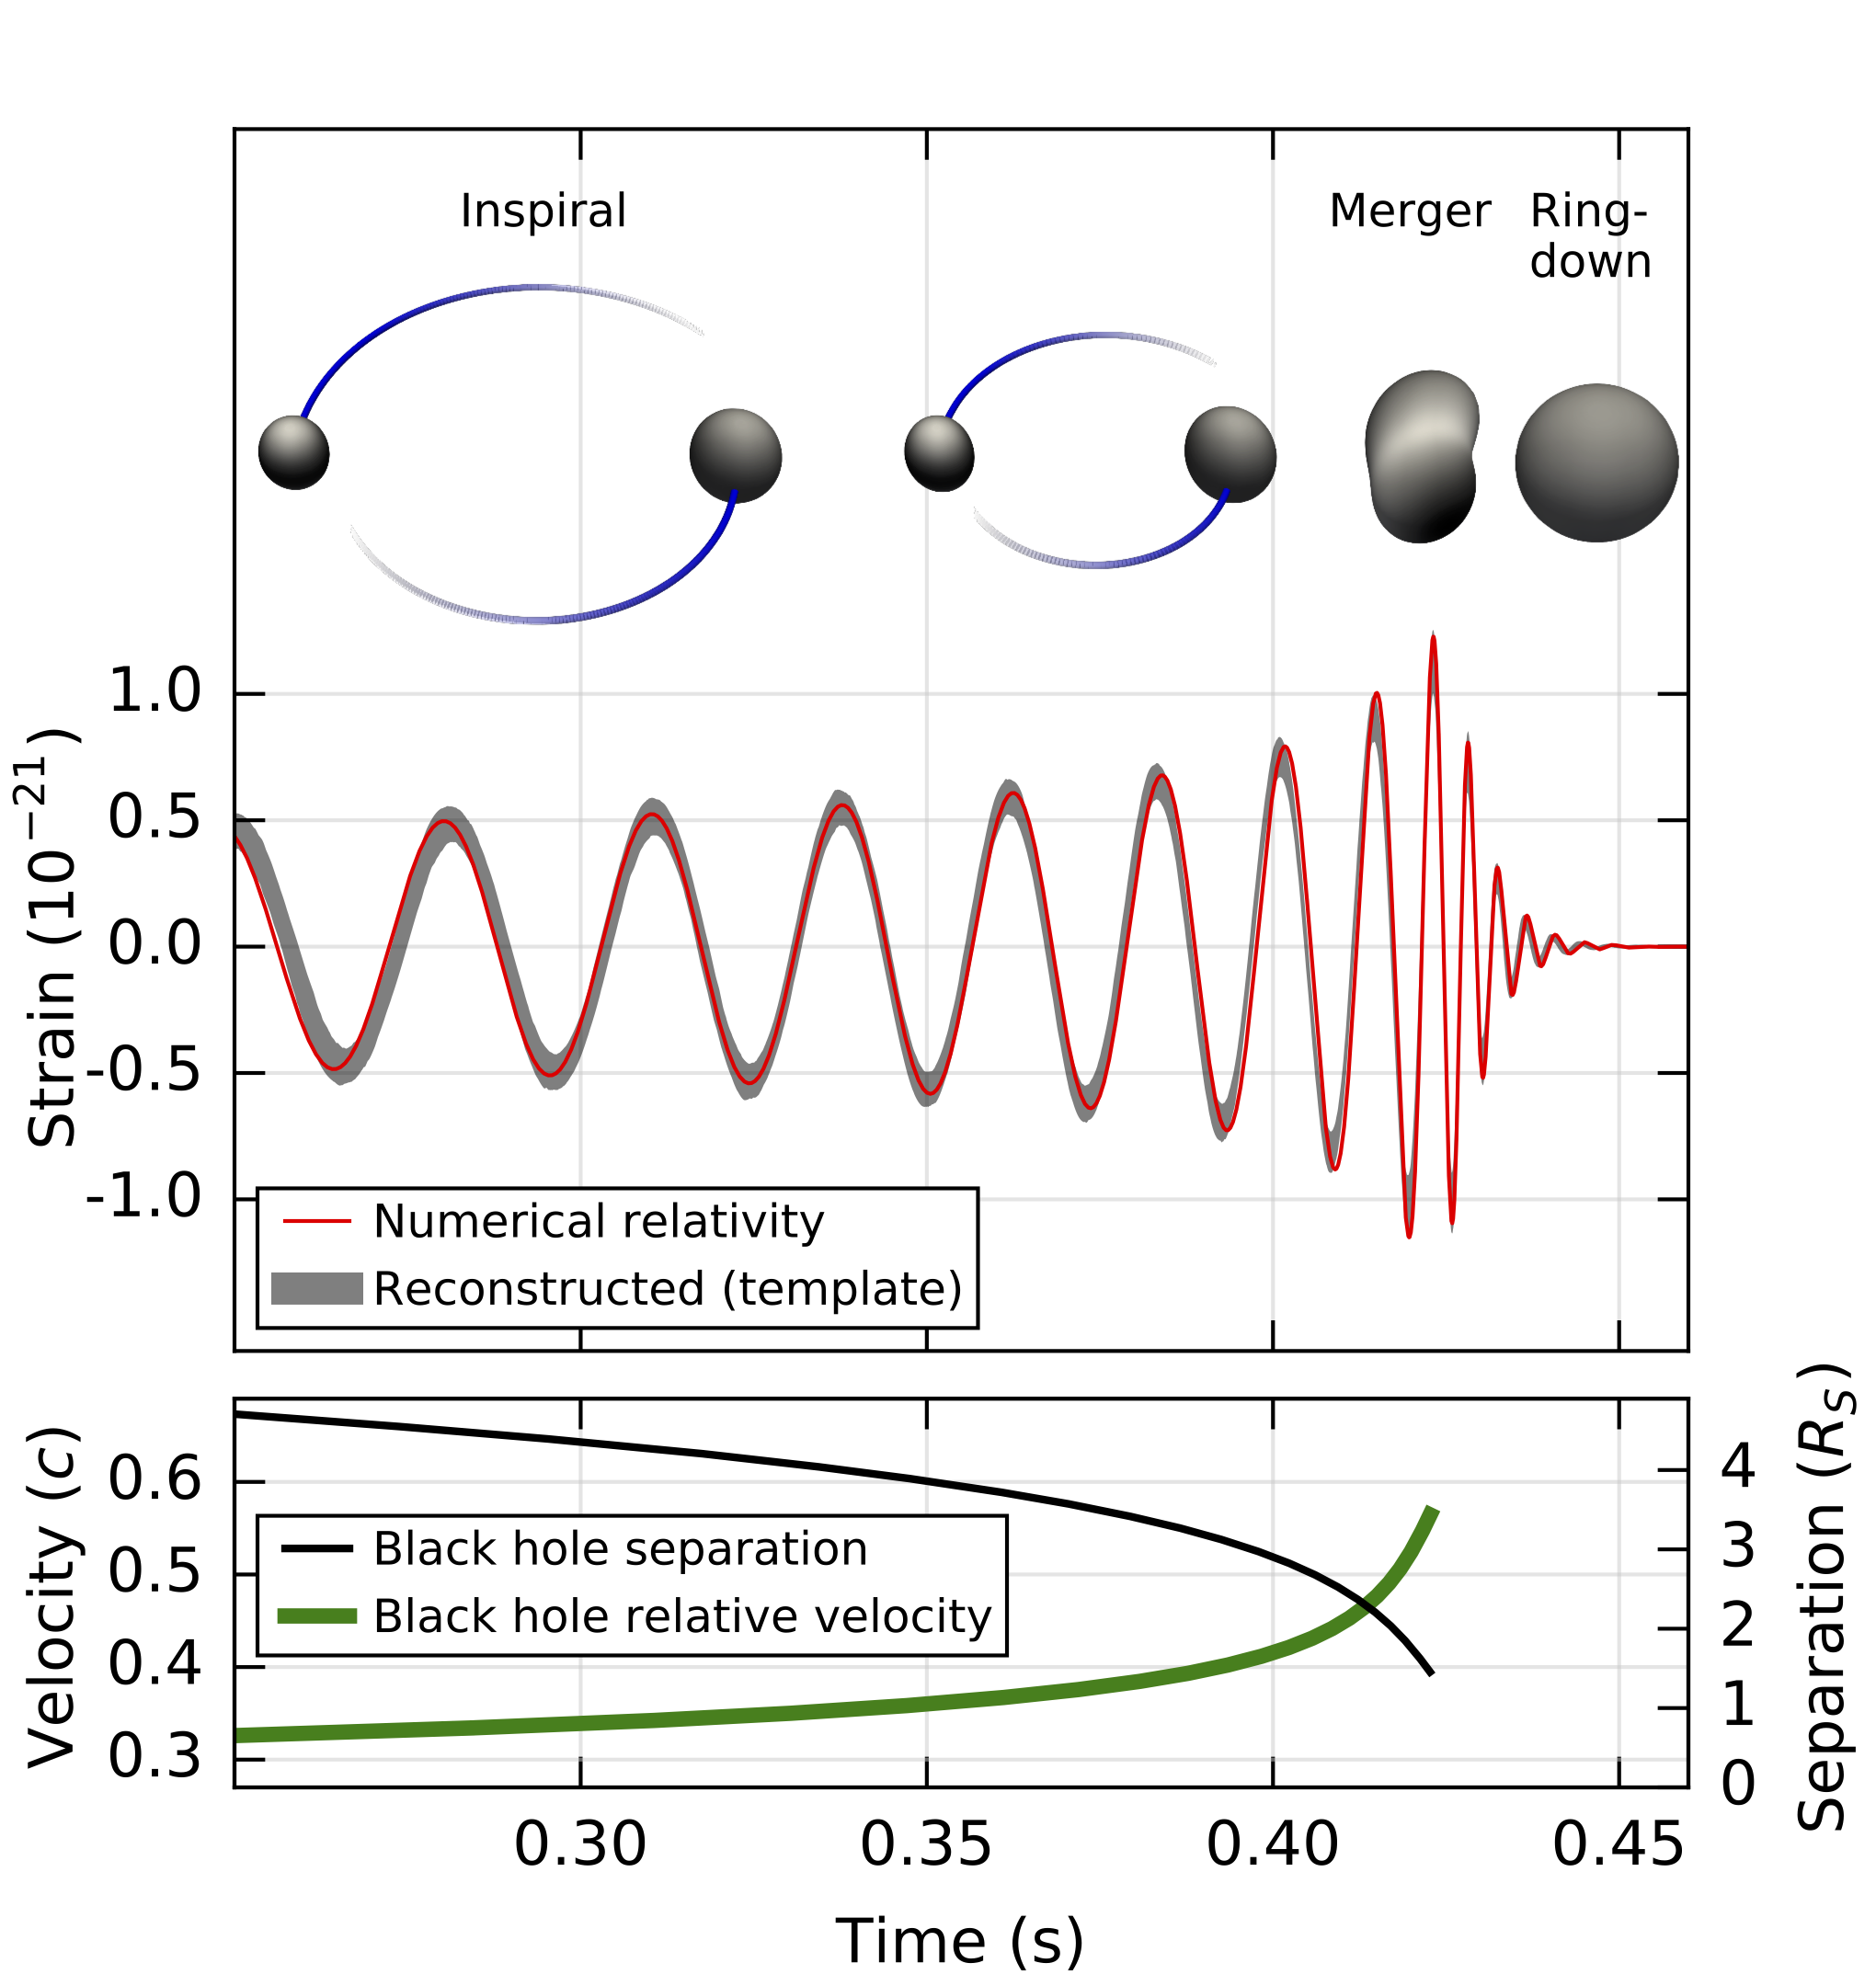
\includegraphics[scale=2]{fig-3.png}
	%\includegraphics[scale=1.2]{../../papers/HigherModes/figs/PNNRMatching_SpEC_q8.pdf}
	\caption{\small{Characteristic morphology of a GW signal from binary black holes. When the black holes are adequately separated in space, their speeds are slow and we can describe the system using analytical approximations; unfortunately, when they are close to each other, their speeds are really high and we have to rely on full numerical simulations to get the form of the GW signal. (Plot from the GW150914 discovery paper)}}
	\label{fig:hybridTD_l2m2}
\end{figure*}


Isolated black holes in general relativity can be uniquely described by their masses and their three-dimensional spins on account of the \textit{no-hair theorem},. Numerical simulations empirically suggest that the \textit{no-hair theorem} should extend to BBHs, and that the dynamics should be uniquely specified using masses and spins of the two black holes.

Alternative exotic proposals to black holes like \textit{boson stars} and \textit{gravastars} exist in the literature. These exotic proposals are only slightly less compact as compared to black holes, but differ from black holes in that they are tidally deformed by their binary companion object. Hence, we expect these objects to have a non-zero tidal deformability parameter $ \Lambda $. For an arbitrary equation of state of the exotic object, there is a theoretical, non-zero lower limit on $ \Lambda $.

\end{textblock}

\begin{textblock}{7}(9,4.2)	% syntax: {colum_width} (x_coordinate, y_coordinate) in inches
\vspace{0.5cm}
\begin{figure*}[t]
	\centering
	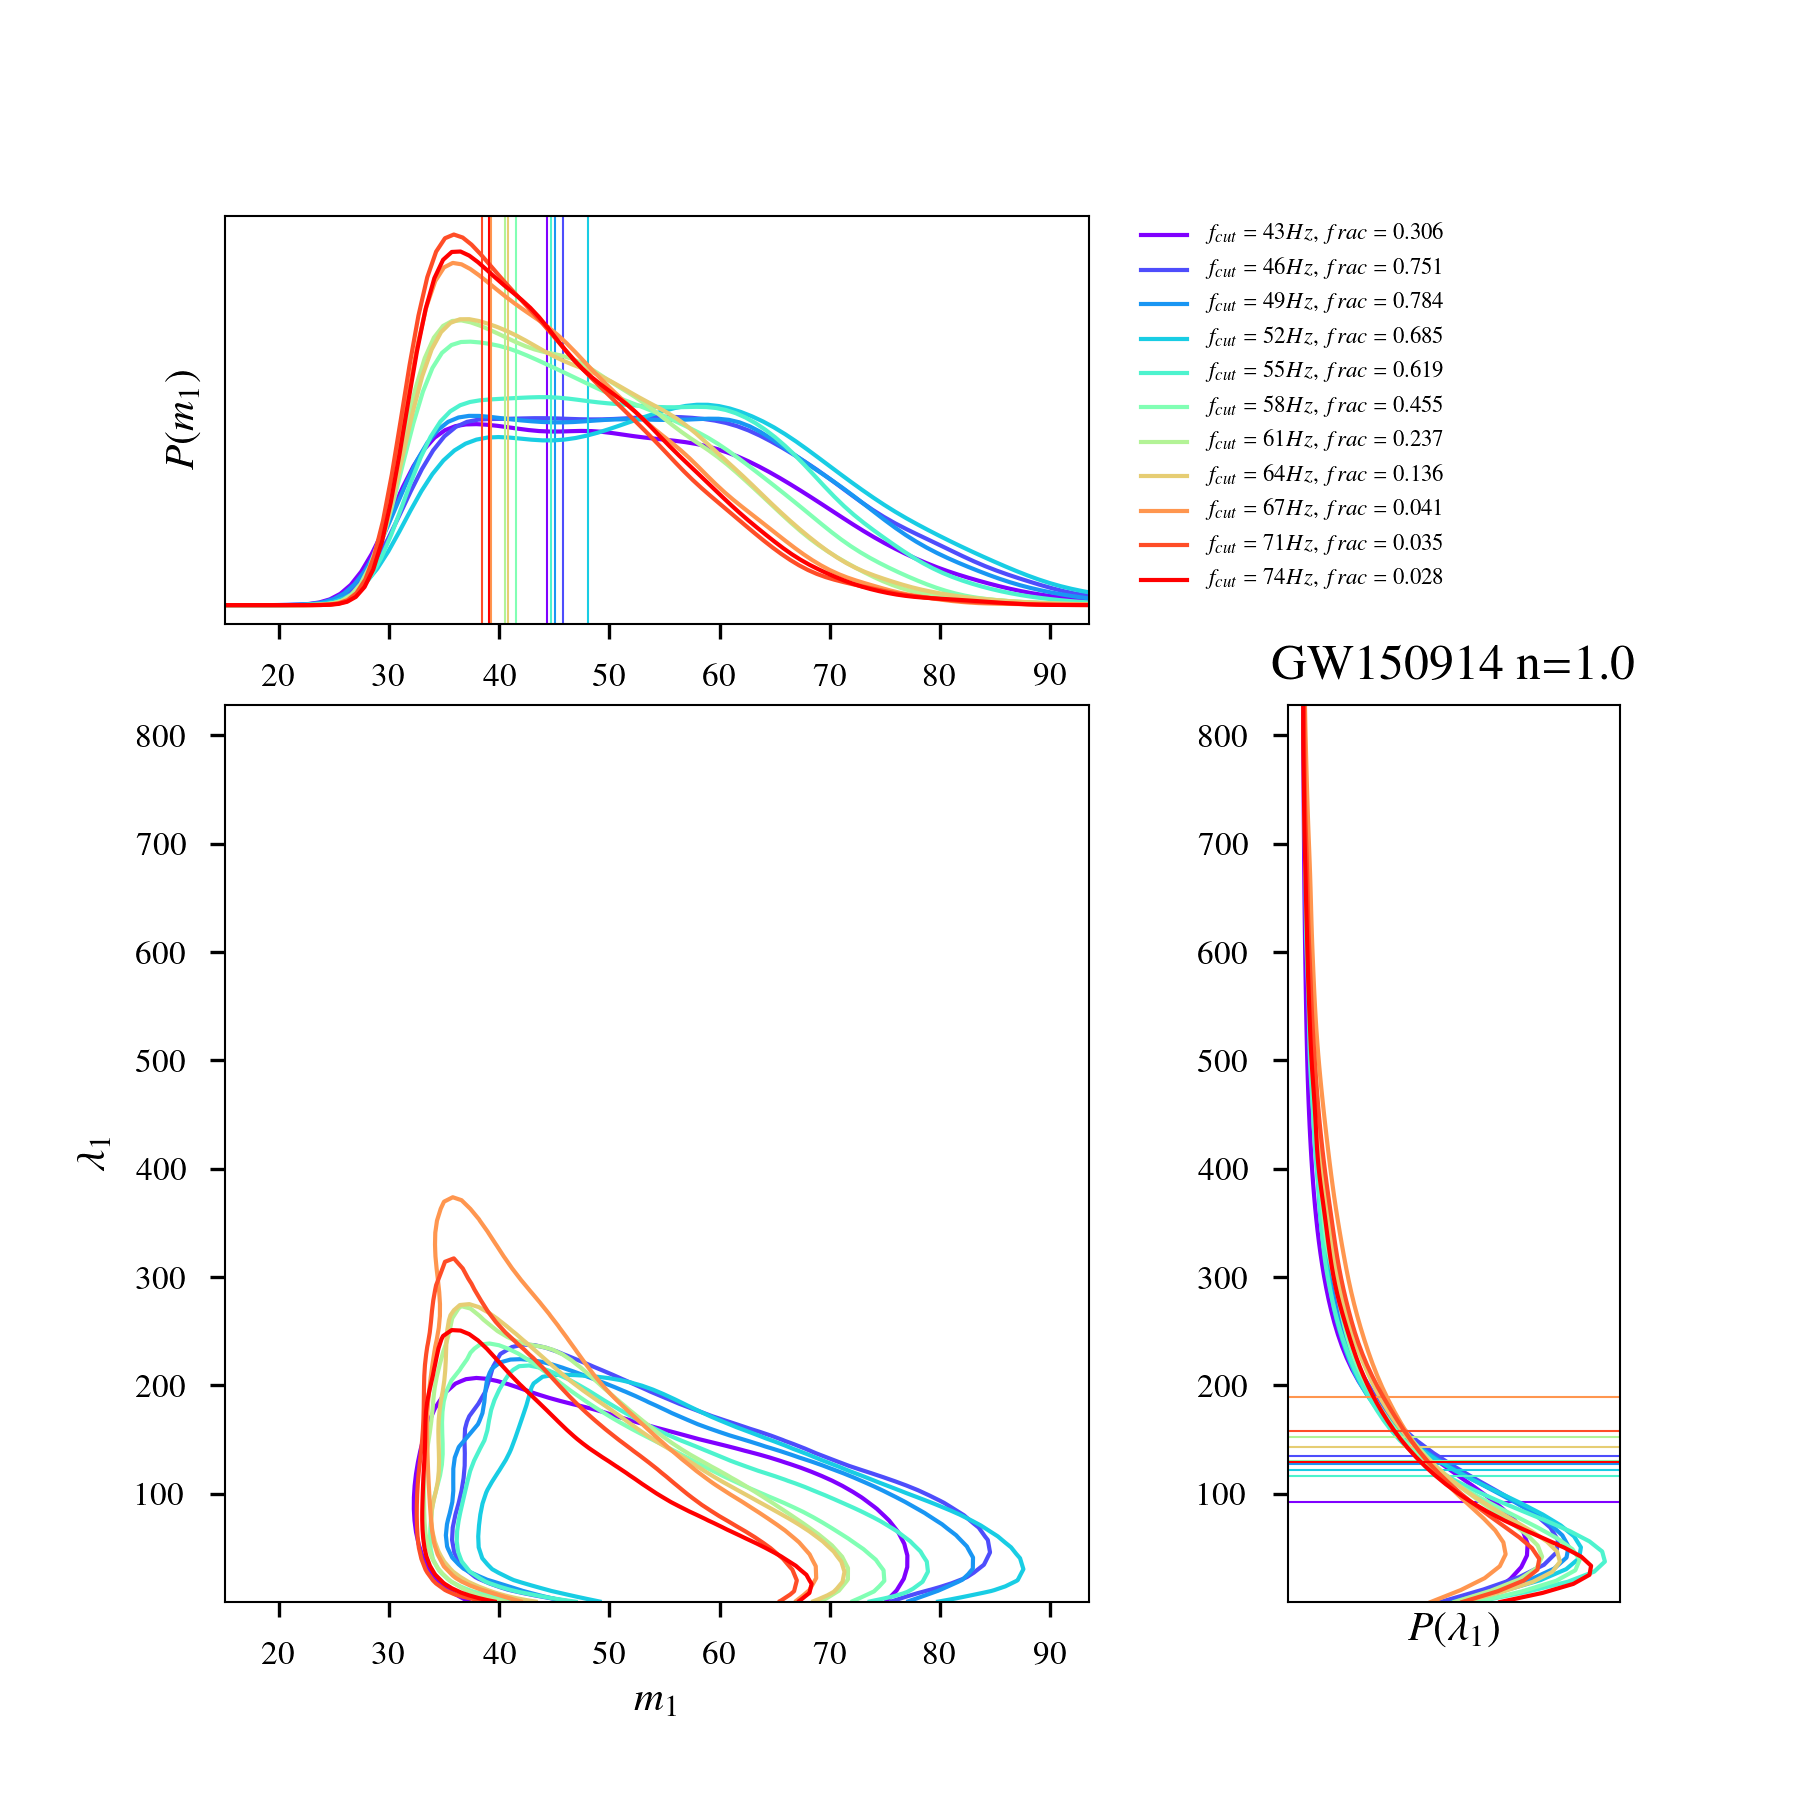
\includegraphics[scale=1.4]{GW150914.png}
	%\includegraphics[scale=1.2]{../../papers/HigherModes/figs/PNNRMatching_SpEC_q8.pdf}
	\caption{\small{Posterior (conditional) distributions of the mass $m_1$ and tidal deformability $\Lambda_1$ of the more massive object (marginalized over all other parameters), obtained from GW150914. The middle panel shows the 68\% credible regions in the marginalized posterior distribution $P (m_1, \Lambda_1)$ while top/side panels show the marginalized one-dimensional posteriors $P(m_1)$ and $P(\Lambda_1)$. The legends show the cutoff frequencies employed in the calculation of these posteriors and the fraction of posterior samples with contact frequency (computed using $n = 1.0$) larger than the cutoff frequency employed. The vertical lines on the top panel show the 68\% credible lower bounds on $m_1$ while the horizontal lines on the side panel show the 68\% credible upper bounds on $\Lambda_1$.}}
	\label{fig:hybridTD_l2m2}
\end{figure*}
\LHead{Method and Results}

\begin{itemize}
	\item Truncate the signal at certain Fourier freqeuncies $ f_{cut} $ before the \textit{merger} regime. Numerical simulations of exotic objects are at a very nascent stage, and hence we cannot accurately model the signal when these objects are close. 
	\item Estimate parameters of the GW signal considering non-spinning objects of tidal deformabilties $ \Lambda_1 $ and $ \Lambda_2 $ using Monte Carlo techniques
	\item Assuming perfect-fluid, non-spinning stars with a polytropic equation of state, calculate the contact frequency $f_{contact}$ for each sample in the estimated conditional distribution.
	\item Choose the $ \Lambda $ measured corresponding to the $ f_{cut} $ value that has maximum fraction of samples satisfying $ f_{contact} > f_{cut} $ as the constraint. Use the measured value of $ \Lambda $ to rule out polytropes.
\end{itemize}

\begin{figure*}[t]
	\centering
	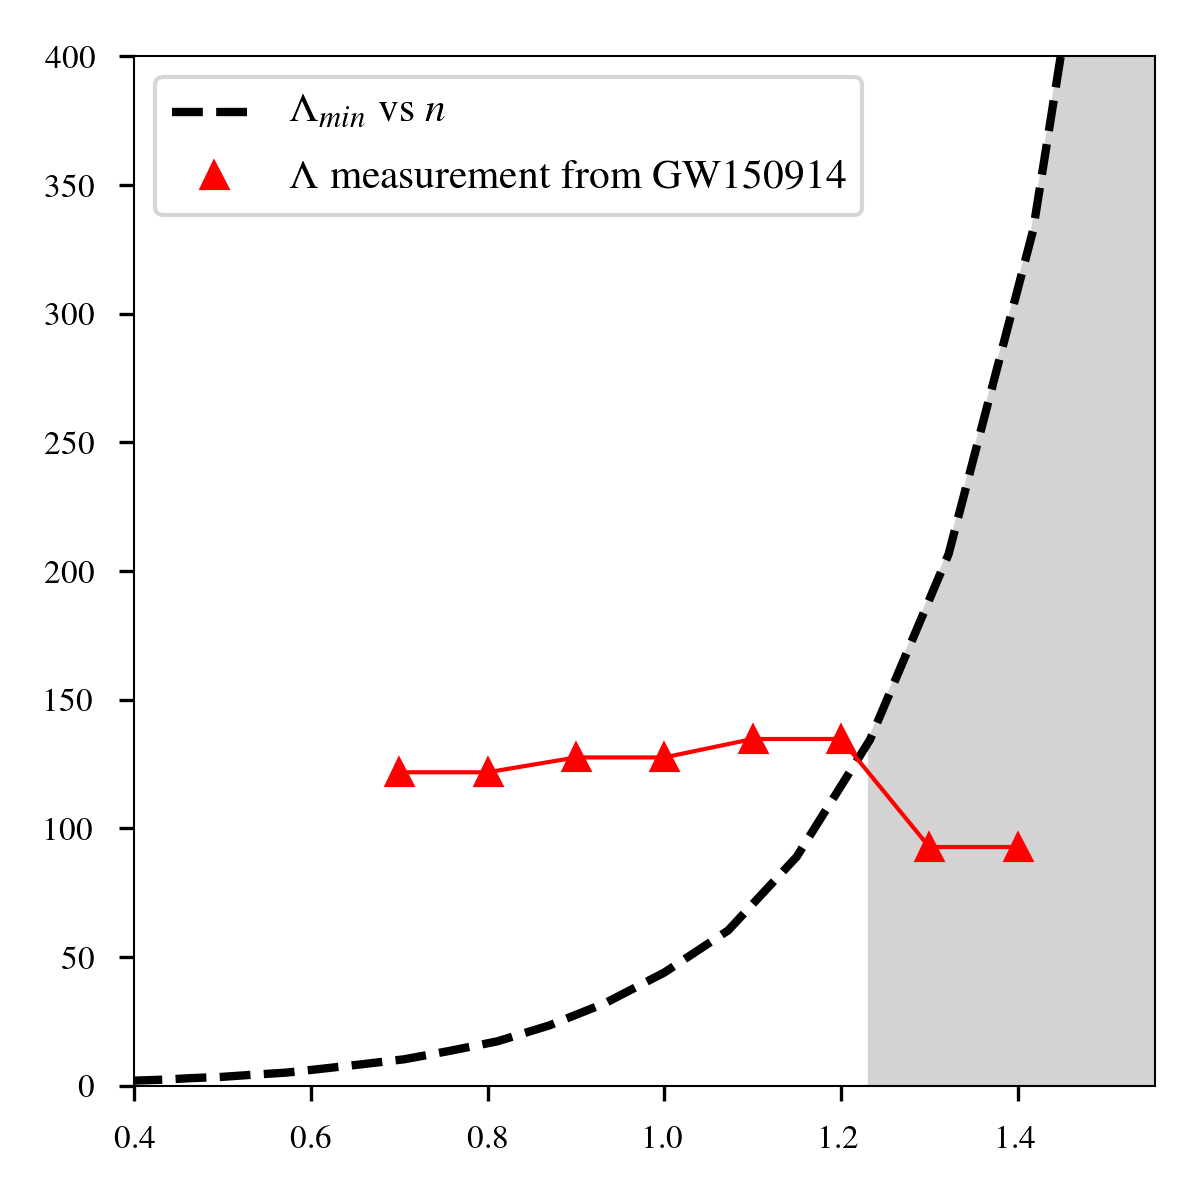
\includegraphics[scale=1.5]{GW150914_68p_constraints.png}
	%\includegraphics[scale=1.2]{../../papers/HigherModes/figs/PNNRMatching_SpEC_q8.pdf}
	\caption{\small{The estimated $\Lambda$ for various polytropic indices. The shaded region corresponds to observed $\Lambda < \Lambda_\mathrm{min}$ (theoretical), and is therefore ruled out by GW150914.}}
\end{figure*}

\end{textblock}

%%%%%%%%%%%%%%%%%%%%%%%%%%%%%%%%%%%%%%%%%%%%%%%%%%%%%%%%%%%%%%%%%%%%%%%%%
%%%%%%%%%%%%%% Place the institute logos at the bottom left %%%%%%%%%%%%
%%%%%%%%%%%%%%%%%%%%%%%%%%%%%%%%%%%%%%%%%%%%%%%%%%%%%%%%%%%%%%%%%%%%%%%%%
\begin{textblock}{18}(1.,23)   
%\resizebox{2\TPHorizModule}{!}{\includegraphics{figs/icts_logo.pdf}} \hspace{1.cm}
%\resizebox{2\TPHorizModule}{!}{\includegraphics{figs/IndigoLogo_crop.png}} \hspace{1.cm}
%\resizebox{0.85\TPHorizModule}{!}{\includegraphics{figs/CardiffLogo.png}} \hspace{1.cm}
%\resizebox{0.85\TPHorizModule}{!}{\includegraphics{figs/logo-UIB.pdf}}
%\resizebox{1\TPHorizModule}{!}{\includegraphics{figs/rri-logo.jpg}}\hspace{1cm}
%\resizebox{1\TPHorizModule}{!}{\includegraphics{figs/cmi-header2.png}}
\end{textblock}
%%%%%%%%%%%%%%%%%%%%%%%%%%%%%%%%%%%%%%%%%%%%%%%%%%%%%%%%%%%%%%%%%%%%%%%%%

%%%%%%%%%%%%%%%%%%%%%%%%%%%%%%%%%%%%%%%%%%%%%%%%%%%%%%%%%%%%%%%%%%%%%%%%%
%%%%%%%%%%%%%%%%%%%%%%%%%%%% Acknowledgments %%%%%%%%%%%%%%%%%%%%%%%%%%%%
%%%%%%%%%%%%%%%%%%%%%%%%%%%%%%%%%%%%%%%%%%%%%%%%%%%%%%%%%%%%%%%%%%%%%%%%%
\begin{textblock}{14}(1.5,24)
\small{\textbf{Acknowledgements} - We would like to thank Krishnendu NV and M Saleem for discussions, and collaboration on a related project. Computations were performed on the \textit{Alice} cluster at ICTS.}

\end{textblock}
%%%%%%%%%%%%%%%%%%%%%%%%%%%%%%%%%%%%%%%%%%%%%%%%%%%%%%%%%%%%%%%%%%%%%%%%%

\end{document}

